\section{Sensitivity of Internally Generated Field to Permeability of the Shield $B_0(\mu)$\label{sec:calculation}}

\subsection{Analytical Calculations in Spherical (and Cylindrical) Geometry}


The presence of a coil inside the innermost passive shield turns the
shield into a return yoke and it is due to the penetration of the
magnetic field flux into the magnetic shield.  The ratio of the
magnetic field inside the coil in the presence of the magnetic shield
to that of the coil in free space is called the reaction factor.
Normally the reaction factor is larger than unity for spherical and
cylindrical geometries.  The key issue of interest for this work is
the dependence of the reaction factor o n $\mu$.  This factor can be
calculated analytically for spherical and cylindrical
geometries~\cite{bib:bidinosti,bib:urankar}.  Although the dependence
of the reaction factor on $\mu$ is rather weak for these geometries,
the constraints on $B_0$ stability are very stringent.  Thus a small
change in the magnetic properties of the innermost shield can result
in an unacceptably large change in $B_0$.

Fig.~\ref{fig:Magnetic_Field} shows the central magnetic field $B_0$
as a function of relative $\mu_r=\mu/\mu_0$ for coil radius 0.53~m
inside a magnetic shield with the inner radius of $0.57$~m and a
thickness of 1.5~mm.  The dimensions have been selected to be
comparable to the dimensions of the ILL nEDM experiment
geometry~\cite{bib:baker,bib:knecht}.
\begin{figure}[h!]
\begin{center}
   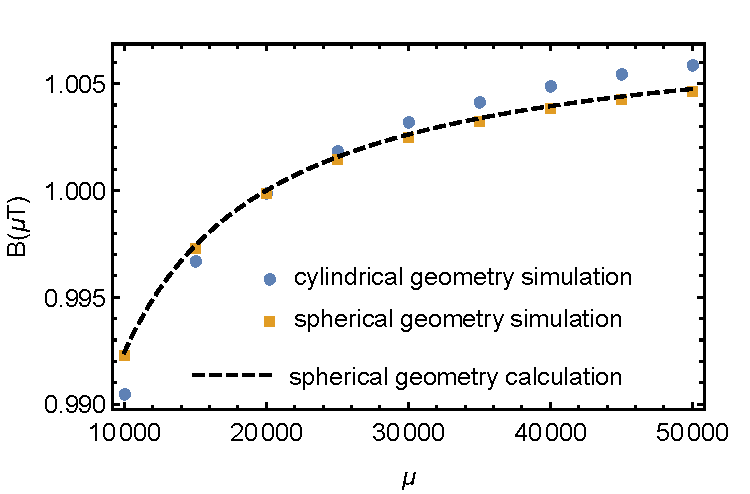
\includegraphics[width=0.7\textwidth]{femm_and_calcs.pdf}
    \caption{Magnetic field as a function of relative magnetic
      permeability $\mu_r$ for geometries similar to the ILL nEDM
      experiment.  The dashed line is for an ideal spherical surface
      current of radius 0.53~m inside a spherical shell of inner
      radius 0.57~m, thickness 1.5~mm.  Open and close circles are
      FEMM-based simulations of spherical and cylindrical geometries
      with similar dimensions, described in the text.  The coil
      currents have been arranged to give a $1~\mu$T field at the
      $\mu_r=20,000$ point.}
    \label{fig:Magnetic_Field}
    \end{center}
\end{figure} 
For a 10\% change in relative $\mu_r$ (from 20,000 to 22,000), the
magnetic field changes by 0.7~nT.



\subsection{Magnetostatic Simulation Results \label{sec:femm}}

Finite-element analysis simulations were conducted to analyze the
effect of discretizing the surface current, and to test the geometry
dependence of the sensitivity of the experiment to changes in $\mu$.
Two axially symmetric simulations were conducted using
FEMM~\cite{bib:femm}.  In the first simulation, the same spherical
geometry was used as for the analytical calculations.  However, the
surface current was discretized to 50 individual circular wires,
inscribed onto a sphere, and equally spaced vertically (i.e.~a
discrete cos$\theta$ coil).  A square wire profile of side length 1~mm
was used.  As shown in Fig.~\ref{fig:Magnetic_Field}, this simulation
gave good agreement with the analytical calculation.

As an example of one additional axially symmetric geometry, a solenoid
within a cylindrical shield was simulated, with equal coil spacings.
In the limit of infinite $\mu$, the image currents in the end caps of
the shield are an infinite series of coils, giving an ideal infinite
solenoid with a uniform field.  Again, fifty discrete coils were
simulated, where the spacing from an end coil to the inner face of the
shield end-cap being half the inter-coil spacing, as appropriate to
generate the correct image currents in the infinite $\mu$ limit. 

As shown in Fig.~\ref{fig:Magnetic_Field}, the slope of $B_0(\mu)$ is
somewhat steeper, and similar in magnitude to the spherical case.  We
therefore estimate that the scale of the sensitivity of a generic nEDM
experiment to global changes in the magnetic permeability is
$\frac{\mu}{B_0}\frac{dB_0}{d\mu}\sim 0.01$.

In the spherical case the reaction factor is 1.39, meaning that the
field generated by the spherical coil is amplified by this
multiplicative factor by the presence of the magnetic shield (flux
return).  In the cylindrical case the reaction factor is 1.35.  If the
reaction factor is closer to unity, the calculated
$\frac{\mu}{B_0}\frac{dB_0}{d\mu}$ will be smaller, and the EDM
experiment less sensitive to changes in $\mu$.  The results in the two
geometries show that there is also geometry dependence.


\subsubsection{Field within the passive flux return for EDM experiments}

For a high-$\mu$ innermost shield, the magnetic field lines emanating
from the coil all return through the shield.  This principle can be
used to estimate the magnetic field internal to the material $B_m$,
and in our studies gave good agreement with FEA-based simulations.
For the cylindrical geometry described in Sec.~\ref{sec:femm}, $B_m$
is largest in the side walls of the solenoidal flux return, attaining
a maximum value of 170~$\mu$T.  If we assume $\mu_r$=20,000, the $H_m$
field is 0.007~A/m.  Typically the shield is degaussed (idealized)
with the internal coil energized.  After degaussing, $B_m$ must be
approximately the same, since all flux returns through the shield.
However, the $H_m$ field must become significantly smaller, as the
material must reside on the ideal magnetization curve in $B_m-H_m$
space.  (For a discussion of the ideal magnetization curve, we refer
the reader to Ref.~\cite{bib:bozorth}.)  In principle, the $H_m$ field
could be reduced by an order of magnitude, depending on the steepness
of the ideal magnetization curve near the origin.  Nonetheless, these
parameters set a scale for the values of $B_m$ and $H_m$ which we
sought to replicate in our experiments reported in
Section~\ref{sec:tdep}.




\subsection{Summary of $B_0(\mu)$ \label{sec:theory_summary}}

For shield-coupled coils, the magnetic field in the region interior to
the coil is coupled to the properties of the magnetic shell which is
caused by the penetration of the magnetic field flux into the shell
material. In a typical nEDM experiment, the sensitivity of the
internal magnetic field to changes in $\mu$ is
$\frac{\mu}{B_0}\frac{dB_0}{d\mu}\sim 0.01$.
% Save for the end: The coupling can be reduced considerably by using
% a self-shielded coil design, which does not couple strongly to the
% innermost magnetic shield.

The field generated in the innermost magnetic shield by a
shield-coupled coil is typically $B_m=170~\mu$T with $H_m<0.007$~A/m.
The field in the nEDM measurement volume, as well as in the magnetic
shield, must be stable for periods of typically hundreds of seconds
(corresponding to frequencies $<0.01$~Hz).  This sets the relevant
measurement scales for magnetic properties that would be most relevant
to nEDM experiment.
